\subsubsection{Vista dei Dati}
il DFD in Figura \vref{fig:messagesddd} rappresenta flow di dati piu importanti dell'applicazione, ovvero i dati corrispondenti alle richieste dei vari servizi, prenotazioni e scambio di messaggi tra pazienti ed amministratori, che servono ``come mezzo di trasporto''\footnote{Ricordiamo che è prerogativa di XP parlare per metafore.} di informazioni tra clienti ed amministratori. Si puo osservare che la comunicazione e indiretta con uno ``storage mediano''. Una generica richiesta viene opportunamente trasformata in un messaggio che viene inserito in DB. Amministratore preleva questi messaggi ed in base al loro contenuto decide operazione da svolgere. Al termine di ogni operazione viene generato un messaggio per informare client dell avvenuta gestione della richiesta ed anche questo viene inserito in DB da dove viene prelevato al login del paziente.

\begin{figure}[!thp]
\centering
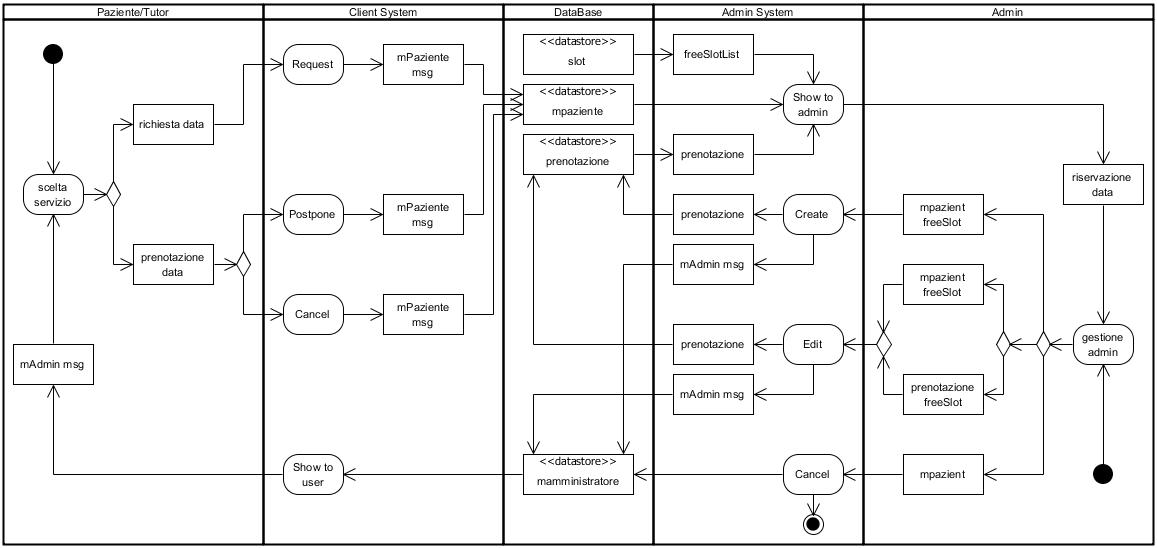
\includegraphics[scale=0.5]{svgs2/ddd/request-prenotation-overall}
\caption{\textit{Messages' Data Flow}.}
\label{fig:messagesddd}
\end{figure}

il DFD in Figura \vref{fig:dvsad}\subref{subfig:tutorreg} rappresenta flow e storage di dati personali dei pazienti mentre DFD in Figura \vref{fig:dvsad}\subref{subfig:tutorreg} rappresenta la stessa cosa in contesto dei dati dei tutor.

\begin{figure}[!thp]
	\centering
	\subfloat[][\emph{Tutor's Registration}.]{\label{subfig:tutorreg}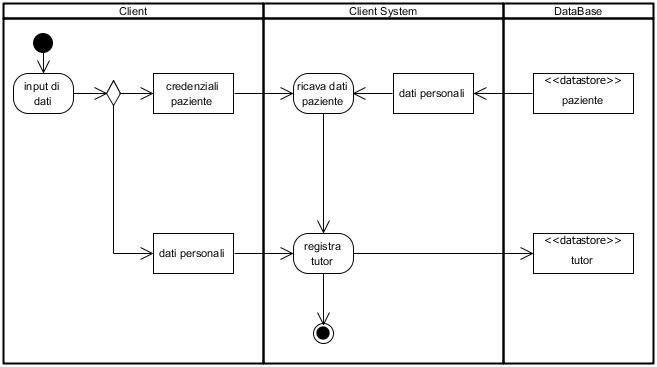
\includegraphics[scale=0.5]{svgs2/ddd/registraT}}\\
	\subfloat[][\emph{Patient's Registration}.]{\label{subfig:tutorreg}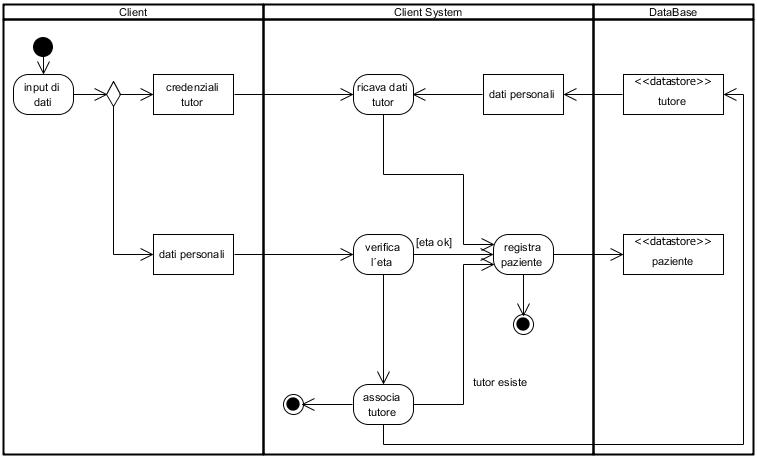
\includegraphics[scale=0.5]{svgs2/ddd/registraP}}\\
	\caption{\textit{User's Data Flow}.}
	\label{fig:dvsad}
\end{figure}


